\documentclass{exam}
\usepackage{graphicx} % Required for inserting images
\usepackage[utf8]{inputenc}
\usepackage[font=normal,labelfont=bf]{caption}
\usepackage{amsfonts}
\usepackage{footnote}
\usepackage{amsmath}
\usepackage{amsthm}
\usepackage{amssymb}
\usepackage{multicol} 
\usepackage{multirow}
\usepackage{rotating}
\usepackage{hyperref}
\usepackage{polynom}
\usepackage{cancel}
\usepackage{colonequals}
\usepackage{answers}
\usepackage{color}
\usepackage{multirow}
\usepackage{tabularx}
\usepackage{float}
\usepackage{tabularx}
\usepackage{indentfirst} %Indents first paragraph after a new section


\pagestyle{headandfoot}
\runningheadrule
\firstpageheader{}{}{}




\runningheader{Mini Project 1}
{}
{}









\newcommand{\bm}{\mathbf}
\newcommand{\E}{\mbox{\rm E}}
\newcommand{\Var}{\mbox{\rm Var}}
\newcommand{\Cov}{\mbox{\rm Cov}}
\newcommand{\PR}{\mathrm{P}}
\newcommand{\y}{\bm{y}}
\newcommand{\X}{\bm{X}}
\newcommand{\be}{\boldsymbol{\beta}}  
\newcommand{\e}{\boldsymbol{\epsilon}}
\newcommand{\R}{\mathbb{R}}





\title{Sport's Players Trends}
\author{Himal Malik}
\date{Due 6/12/2024}

\begin{document}

\maketitle



\section{Executive Summary}
There are 537 rows of data comprising of 11 seasons of data with season 0 being a baseline data for the players. This dataset includes the sports they play, the country they play for and other various data about their statistics such as age, gender, etc. In addition, there is a player value associated with each person so we can track each player's progress across the season.


\section{Figures}
When looking at the different variables some of the key hypothesises that I had about the data was that a greater amount of training hours resulted in a greater player value and that the older you are the more likely your player value will become across the seasons. Instead of looking at all 50 players and how they have changed, I will have a random sample of 10 players from each section I look at.

\subsection{Overall}
Taking a random sample of 10 people

\begin{figure}[h]
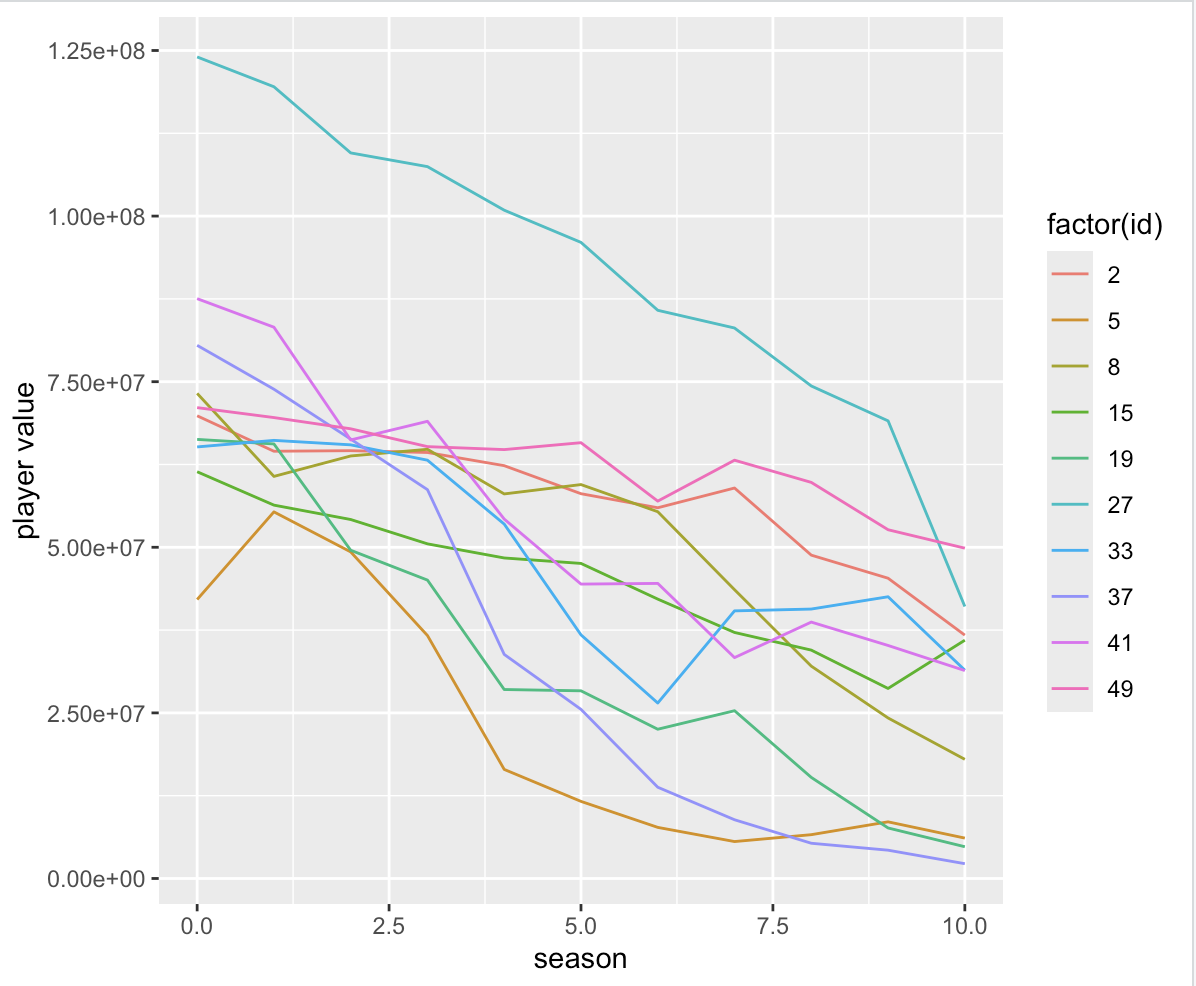
\includegraphics[scale = .5]{Overall.png}
\centering
\end{figure}

\subsection{Age}
Age with 25 as a baseline

\begin{figure}[h]
  \centering
  \begin{minipage}[b]{0.45\textwidth}
    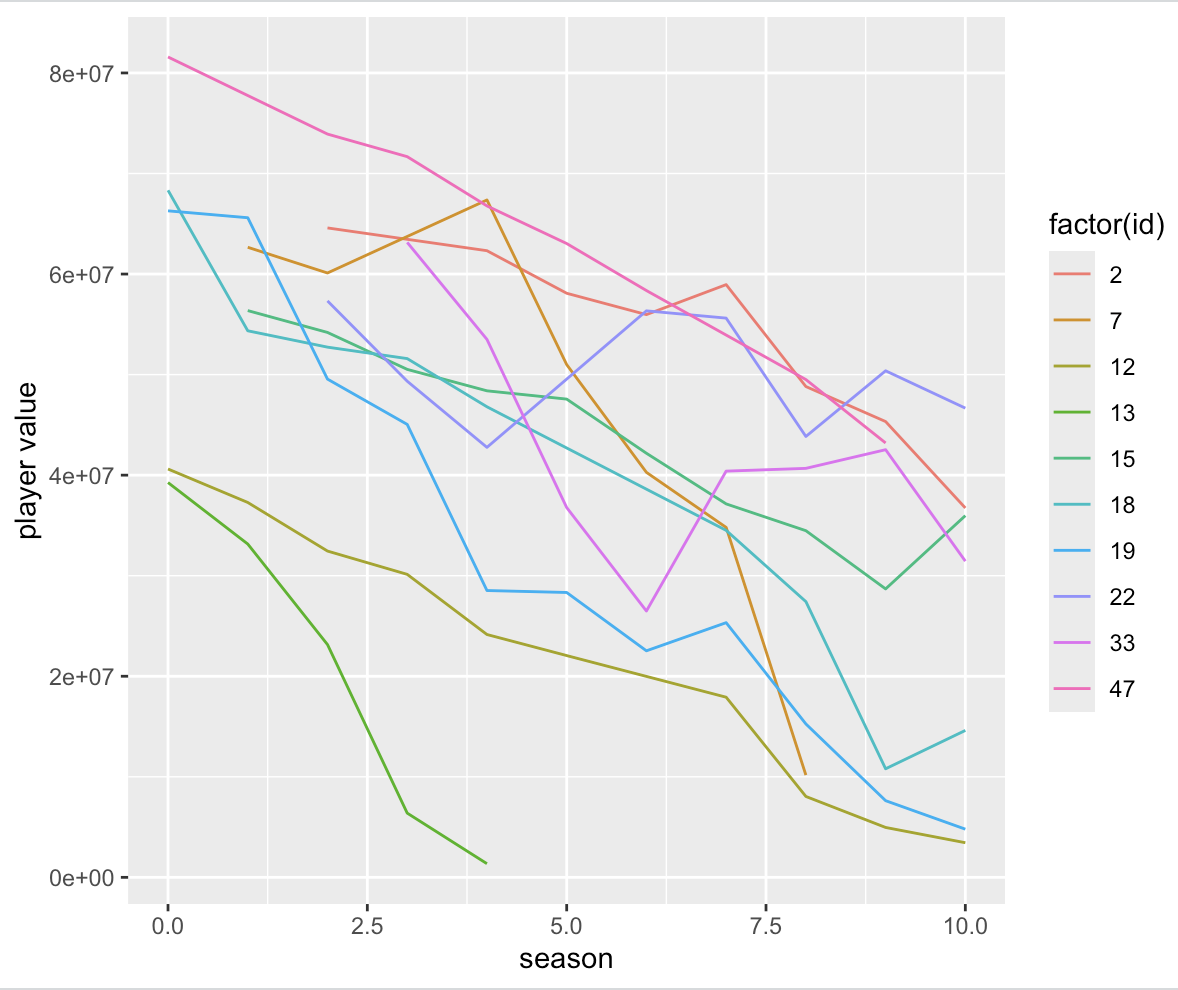
\includegraphics[width=\textwidth]{Older_age.png}
    \caption{Older than 25}
  \end{minipage}
  \hfill
  \begin{minipage}[b]{0.45\textwidth}
    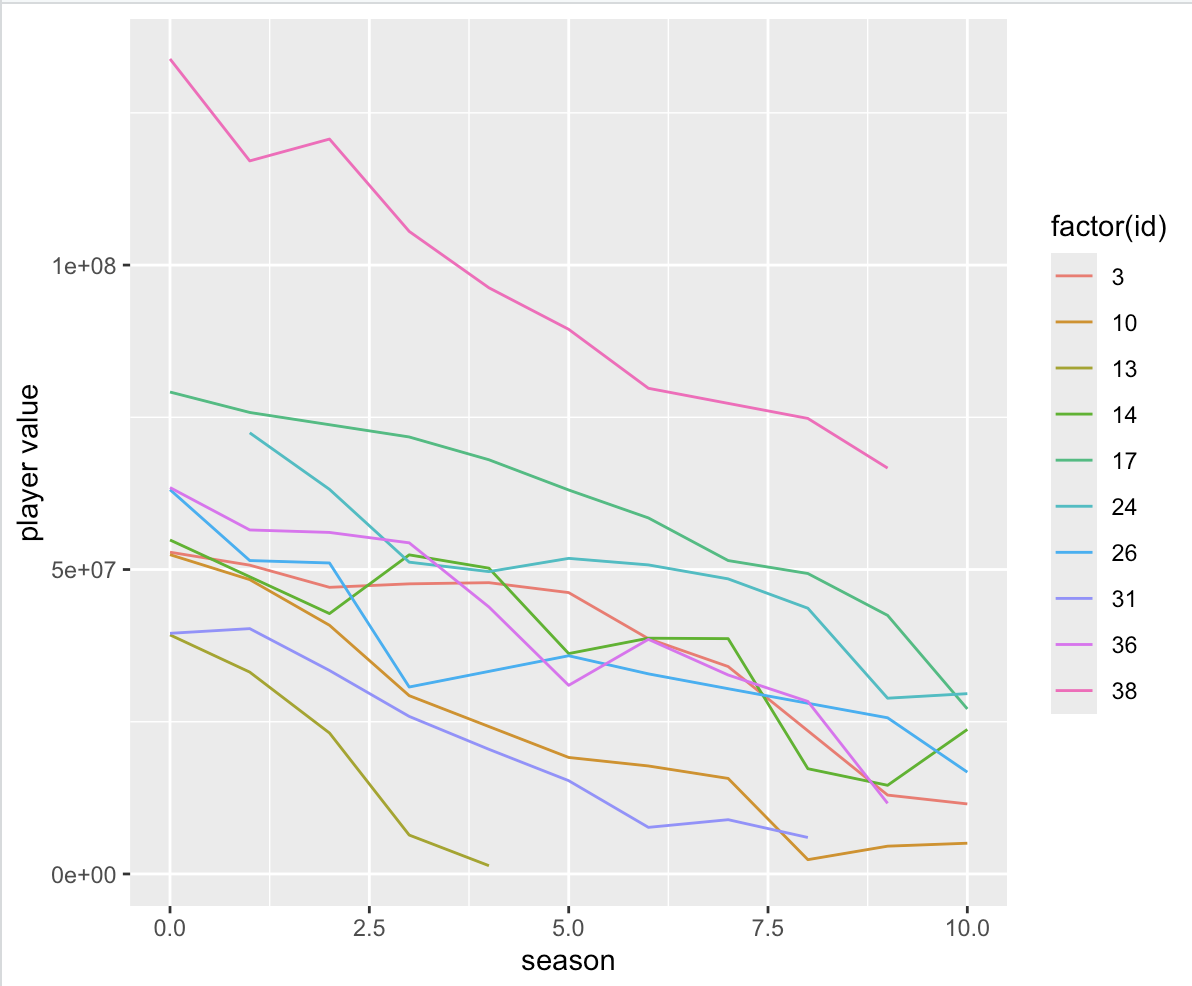
\includegraphics[width=\textwidth]{Younger_age.png}
    \caption{Younger than 25}
  \end{minipage}
\end{figure}

\subsection{Training Hours}
Training Hours with 38 hours as a middle ground

\begin{figure}[h]
  \centering
  \begin{minipage}[b]{0.45\textwidth}
    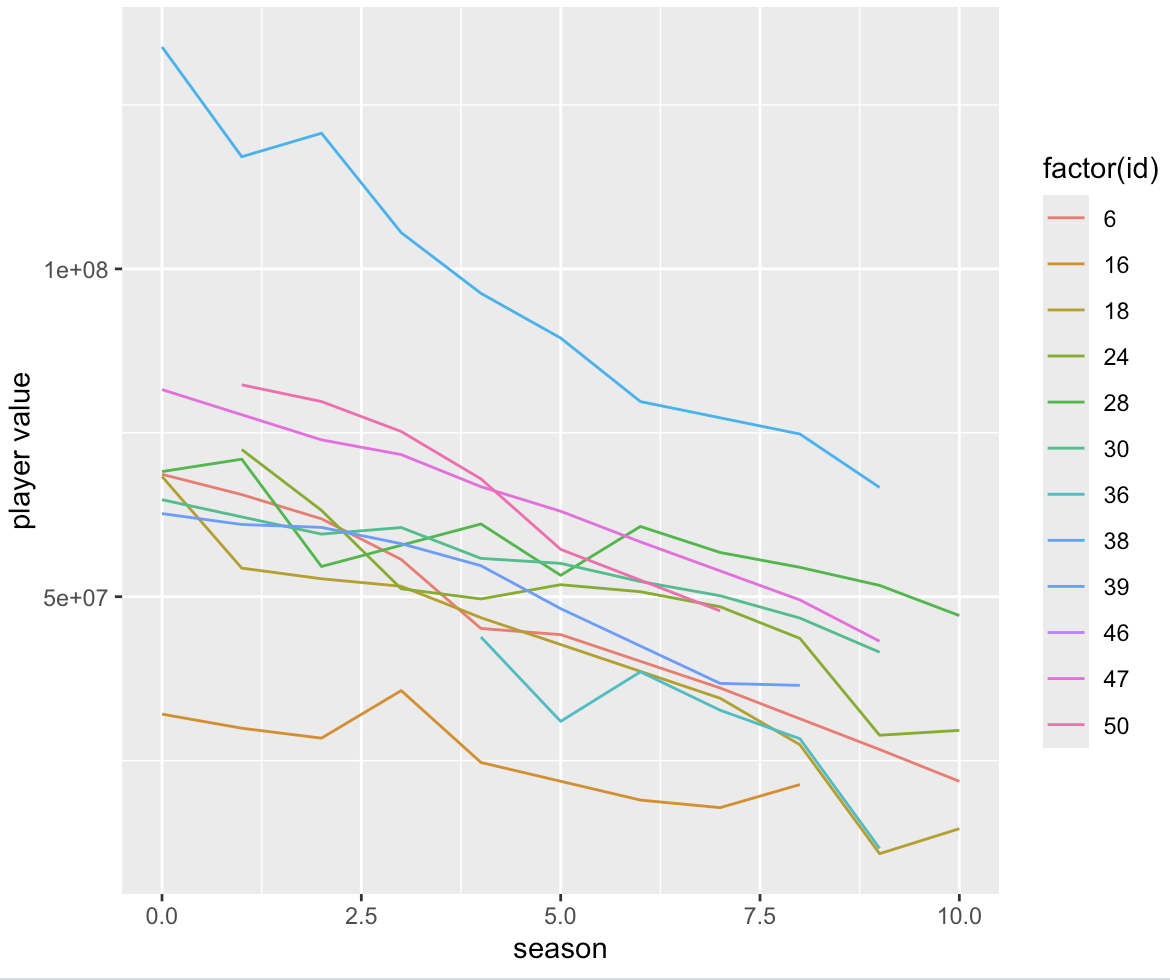
\includegraphics[width=\textwidth]{More Training Hours.png}
    \caption{More Training (greater than 38 hours)}
  \end{minipage}
  \hfill
  \begin{minipage}[b]{0.45\textwidth}
    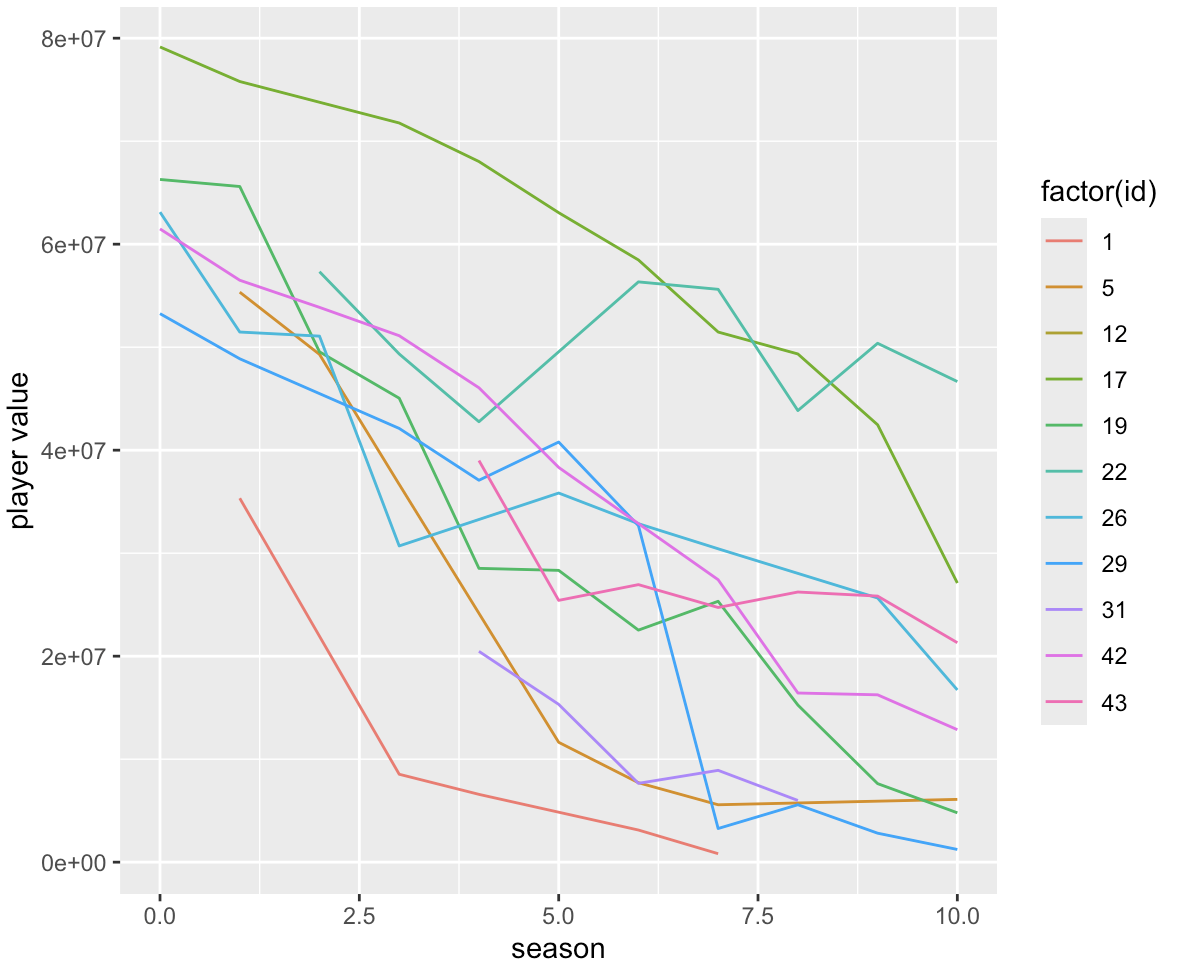
\includegraphics[width=\textwidth]{Less Training Hours.png}
    \caption{Less Training (less than 38 hours)}
  \end{minipage}
\end{figure}


\section{Next Steps}
While the information is comprehensive about the player, there is no information on how well they perform other than the player value. I would want to access their win rate, how many wins/losses they have accumulated across ten games. This way we can make connections with the other given categories. For example, does an increase in training hours mean an increase in their wins and a decrease in their losses. Or does an increase in training hours mean an increase in the player value.

\section{Data/Appendix}
When looking at the baseline data of season 0 there are 50 values with a couple NA values in each respective category but not enough to skew the data. But the most important thing is that there is a consistent amount of 50 players so we can see how much the amount fluctuates.

When looking at the overall data, there is a strong negative correlation between season and player value indicating that as the season goes on, the average player value decreases. 


\subsection{Location}
When looking at the different locations, there was no significant difference from the overall difference in player value. For example, in the USA all the player values consistently decrease.

\begin{figure}[h]
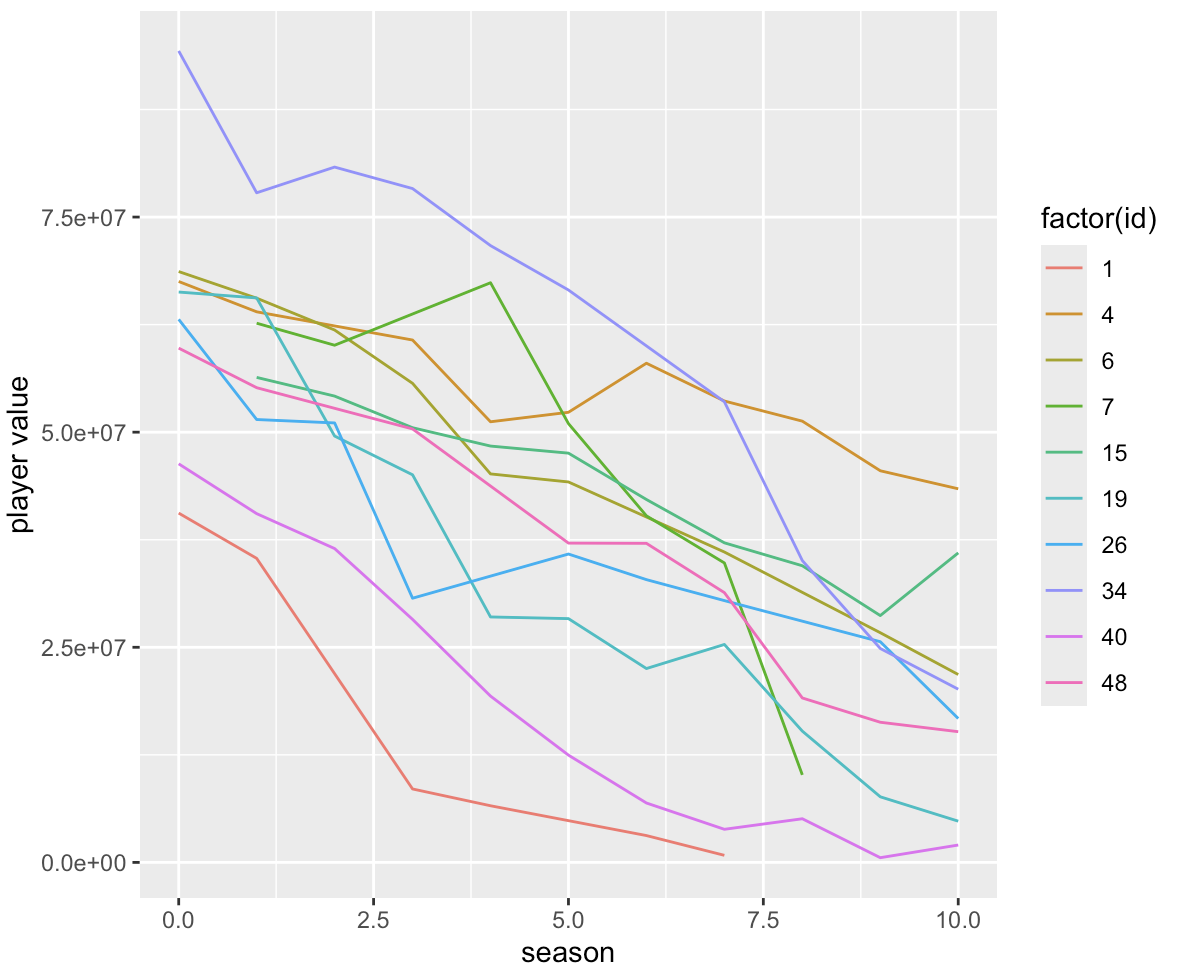
\includegraphics[scale = .6]{USA.png}
\centering
\end{figure}

\newpage
\subsection{Sport}
When looking at the different sports, there was no significant difference from the overall difference in the player value. Take for example football where the player value is consistently decreasing across all the seasons.

\begin{figure}[h]
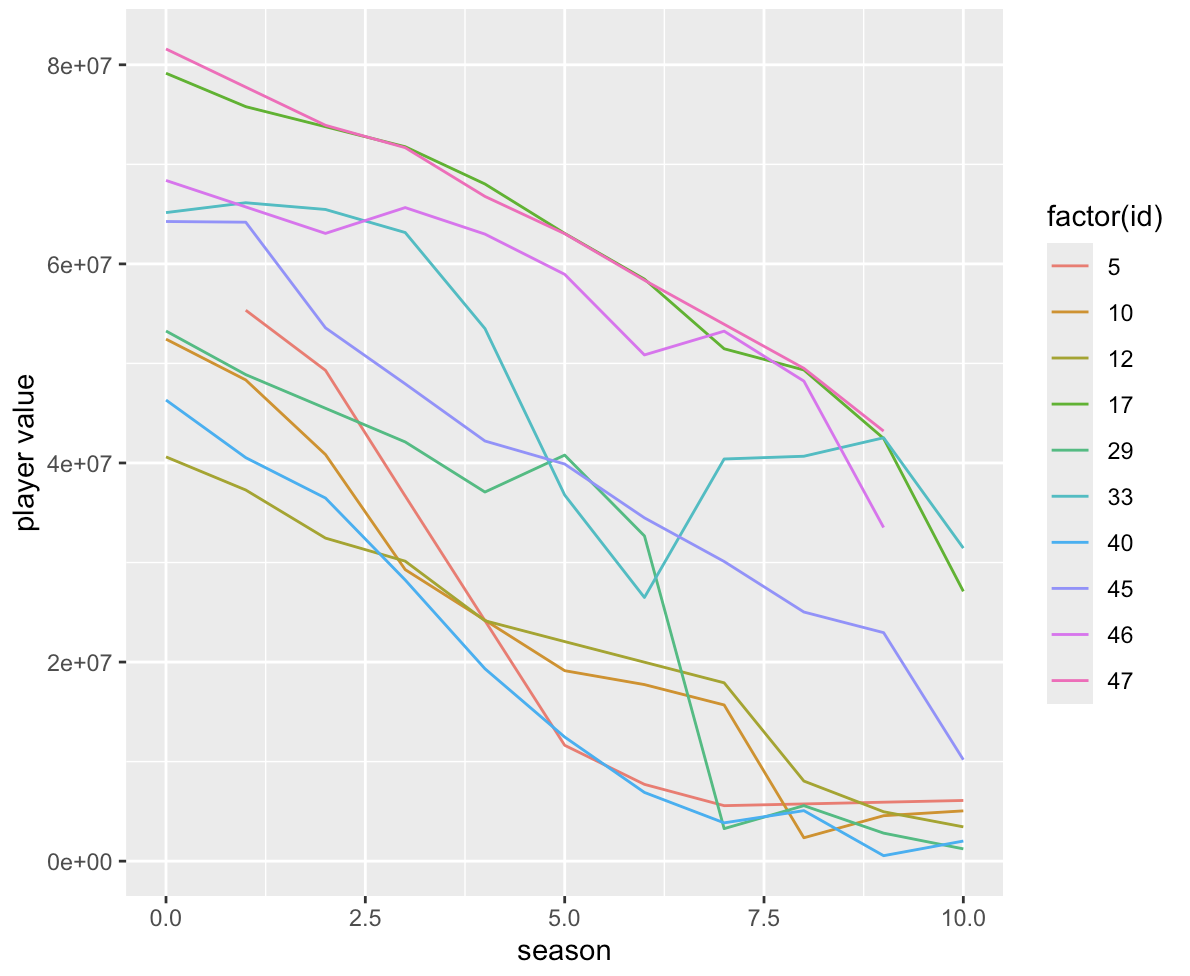
\includegraphics[scale = .5]{Football.png}
\centering
\end{figure}

\subsection{Gender}
When looking at the gender, there was a slight difference in how much the player value dropped. Female's player's values tended to be more consistent than males with males sometimes having their player value drop 50 million dollars over the course of 10 seasons while females will have their value drop at a maximum of 25 million over the course of 10 seasons. 

\begin{figure}[h]
  \centering
  \begin{minipage}[b]{0.45\textwidth}
    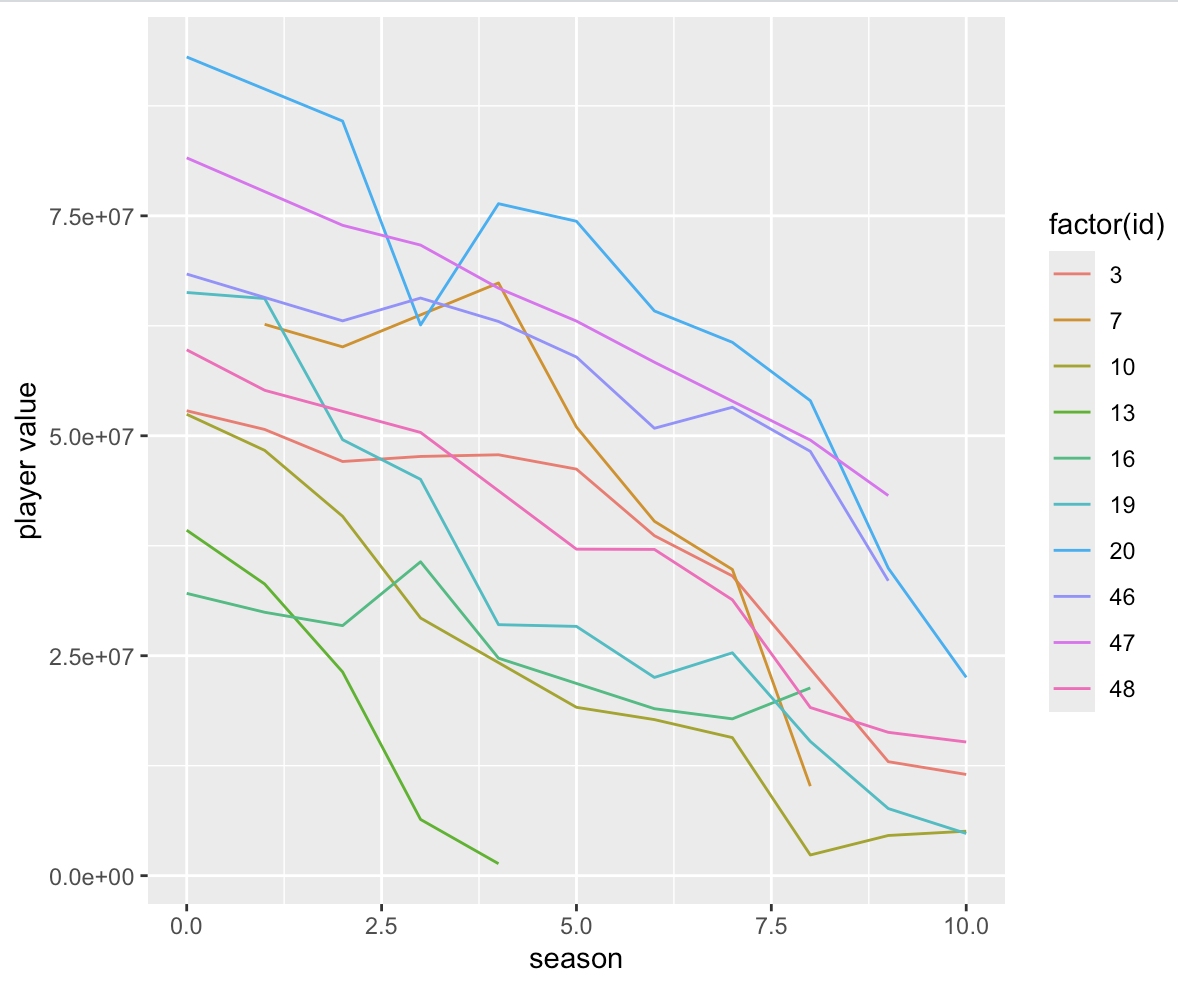
\includegraphics[width=\textwidth]{Male.png}
    \caption{Male}
  \end{minipage}
  \hfill
  \begin{minipage}[b]{0.45\textwidth}
    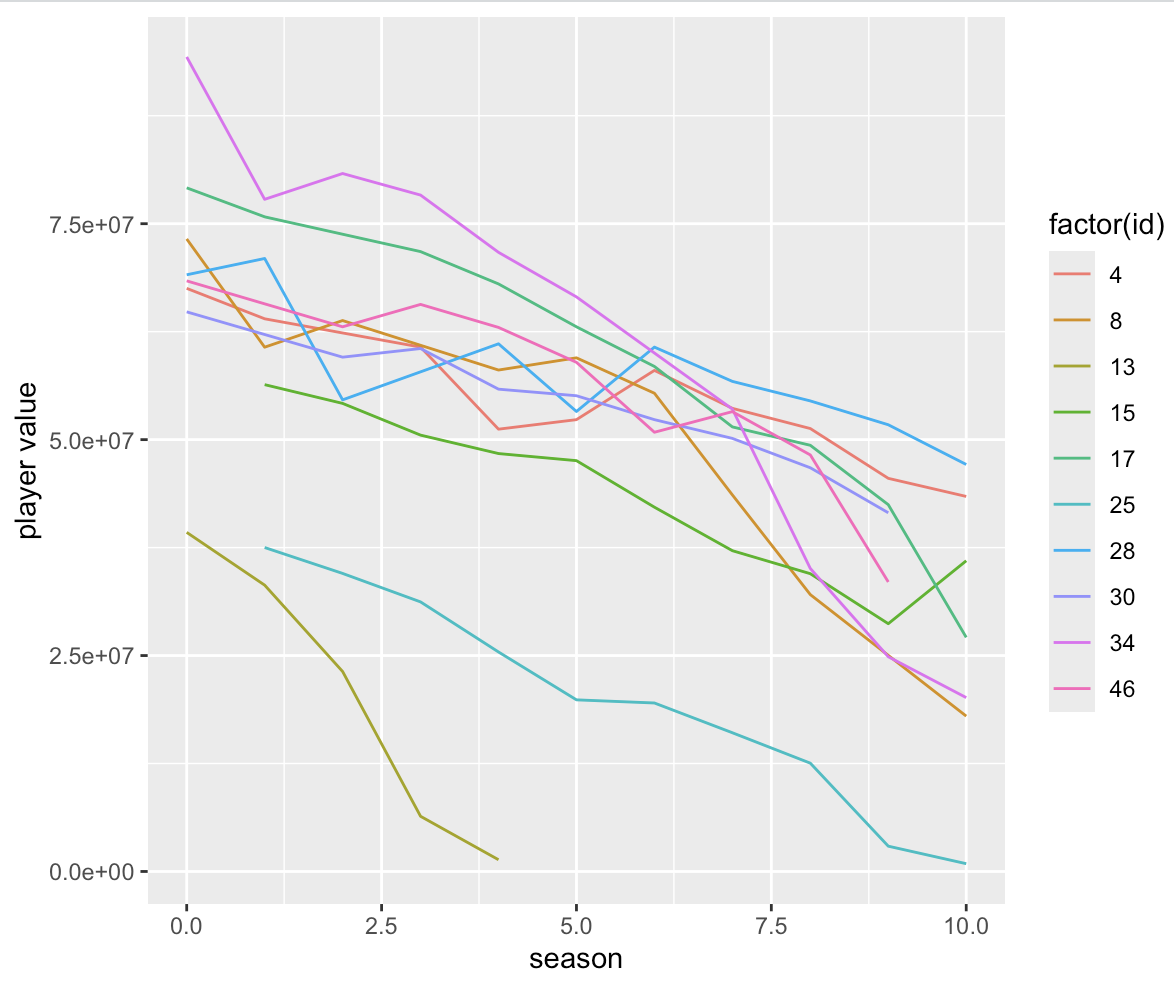
\includegraphics[width=\textwidth]{Female.png}
    \caption{Female}
  \end{minipage}
\end{figure}

\subsection{Results/Conclusion}
The variables that tended to impact player value was most often gender, age, and training hours. Male players tended to have their results more inconsistent compared to females. Players who were older were more likely to male less as the seasons went on with younger players having less of a downward spike in player value. And finally more training hours resulted in a player's value dropping less than the overall while less training hours matched with the overall trend of decreasing player value over 10 seasons.

\end{document}
